\chapter{La Política Comercial Internacional e Instituciones}

\section{Introducción}

Esta área del conocimiento se enfoca en las diversas acciones que los gobiernos adoptan en relación con el comercio internacional.

\subsection{Contextualización de la Política Comercial Internacional}

El análisis de la política comercial se inscribe en la primera parte de la disciplina de la economía internacional, conocida como el análisis del comercio internacional, que se centra en las transacciones reales de la economía global, como el movimiento físico de bienes y servicios. En esta sección se establecen los fundamentos teóricos que explican las ganancias del comercio y los patrones de intercambio, basándose en conceptos como la ventaja comparativa.

Mientras que los fundamentos teóricos demuestran que el comercio internacional puede ser mutuamente beneficioso para las naciones, la política comercial surge como respuesta a la histórica y persistente oposición al librecambio y a la competencia internacional, impulsada a menudo por las preocupaciones sobre el efecto en las industrias nacionales.

\subsection{Instrumentos y Focos de la Intervención}

La política comercial implica la adopción de diversas medidas de intervención, cuyo análisis es fundamental para comprender los efectos sobre el bienestar nacional y la distribución de la renta. Los instrumentos principales se clasifican en dos grandes categorías:
\begin{enumerate}[label=\arabic*)]
    \item \textbf{Instrumentos Arancelarios}: Un \textbf{arancel} es un impuesto que grava un bien cuando cruza las fronteras, típicamente una importación. Históricamente, los aranceles han servido como fuente de ingresos para los estados y, fundamentalmente, para proteger sectores nacionales específicos de la competencia externa. Los instrumentos arancelarios incluyen los aranceles fijos, los aranceles \textit{ad valorem} y los aranceles compuestos.
    \item \textbf{Barreras No Arancelarias (BNA)}: Agrupan una diversidad de medidas que restringen el comercio distintas a los aranceles, y han ganado importancia a medida que los aranceles han disminuido. Las BNA incluyen cuotas de importación (límites a la cantidad de importaciones), restricciones voluntarias a la exportación (RVE), subsidios a la exportación, exigencias de contenido nacional, políticas de adquisición gubernamental, y regulaciones técnicas o sanitarias.
\end{enumerate}

\subsection{El Debate Central y las Instituciones Globales}

Un tema perenne en la economía internacional es el debate entre el \textbf{librecambio} y el \textbf{proteccionismo}. Aunque los economistas suelen defender el librecambio por sus beneficios de eficiencia y ganancias adicionales, la intervención se justifica a menudo basándose en argumentos como la explotación del poder de mercado nacional para mejorar la \textbf{relación de intercambio} (arancel óptimo) o la corrección de fallos específicos del mercado.

Para coordinar las políticas comerciales y avanzar hacia la liberalización del comercio, se han establecido acuerdos y organizaciones internacionales. La liberalización comercial se ha fundamentado históricamente en acuerdos \textbf{multilaterales}, en particular, bajo el marco del \textbf{Acuerdo General sobre Aranceles y Comercio (GATT)}. El GATT, que se basó en el principio de no discriminación y promovió la reducción arancelaria recíproca, fue sustituido formalmente por la \textbf{Organización Mundial del Comercio (OMC)} en 1995. La OMC amplió el alcance del sistema multilateral, incluyendo el comercio de servicios y la propiedad intelectual, y fortaleció el mecanismo de resolución de disputas comerciales entre sus miembros.

El estudio de la política comercial internacional también aborda cuestiones contemporáneas como la \textbf{política comercial estratégica} en mercados de competencia imperfecta, el impacto de la globalización sobre los salarios y el medio ambiente, y las políticas comerciales específicas adoptadas por los países en desarrollo, como la industrialización mediante la sustitución de importaciones o la promoción de exportaciones.

\section{Beneficios del Libre Comercio }

El objetivo fundamental de la teoría del comercio es demostrar los beneficios inherentes al libre comercio, los cuales se analizan comúnmente a partir de las curvas de oferta y demanda, y la consiguiente variación de los excedentes del consumidor y del productor . La defensa del libre comercio se sustenta en la \textbf{eliminación de las pérdidas de eficiencia} que conlleva el proteccionismo .

\subsection{Excedente del Consumidor y del Productor }

\subsubsection{Excedente del Consumidor ($\text{EC}$)}
El excedente del consumidor se define como la \textbf{diferencia} entre la cantidad que los compradores estarían dispuestos y serían capaces de pagar por un producto, y la cantidad que realmente pagan . Mide la \textbf{satisfacción} obtenida por el consumidor por encima del precio de mercado . Gráficamente, el $\text{EC}$ se representa por el \textbf{área bajo la curva de la demanda y por encima del precio de mercado} del producto . Una disminución en el precio de mercado lleva a un aumento del $\text{EC}$ .

\subsubsection{Excedente del Productor ($\text{EP}$)}
El excedente del productor es el ingreso que los productores reciben \textbf{por encima de la cantidad mínima requerida} para inducirlos a ofrecer el producto . Esta cantidad mínima debe cubrir los costes variables totales . En términos de factores de producción, el $\text{EP}$ es igual al rendimiento de los factores fijos, equivalente a los ingresos por venta menos el coste variable de producción . Gráficamente, se representa por el \textbf{área por encima de la curva de la oferta y por debajo del precio de mercado} del producto .


\begin{figure}[H]
\centering
% Gráfico de la Izquierda: Excedente del Consumidor
\begin{tikzpicture}[scale=1.2]
    % Ejes
    \draw[->, thick] (0,0) -- (5,0) node[below] {$Q$};
    \draw[->, thick] (0,0) -- (0,5) node[left] {$p$};
    \node at (0, -0.2) {0};

    % Curva de Demanda (D)
    \draw[blue, thick] (0, 4.5) -- (4.5, 0) node[below right] {D};

    % Precios y Cantidades
    \def\pOne{2}
    \def\pTwo{3.5}
    \def\qdOne{2.5}
    \def\qdTwo{1}

    \coordinate (P1_Qd1) at (\qdOne, \pOne);
    \coordinate (P2_Qd2) at (\qdTwo, \pTwo);

    % Líneas discontinuas
    \draw[dashed] (0, \pOne) node[left] {$p_1$} -- (P1_Qd1);
    \draw[dashed] (P1_Qd1) -- (\qdOne, 0) node[below] {$Q_{D1}$};
    
    \draw[dashed] (0, \pTwo) node[left] {$p_2$} -- (P2_Qd2);
    \draw[dashed] (P2_Qd2) -- (\qdTwo, 0) node[below] {$Q_{D2}$};

    % Área del Excedente del Consumidor (EC)
    \coordinate (yInterceptD) at (0, 4.5);
    \fill[blue!20, opacity=0.8] (yInterceptD) -- (P1_Qd1) -- (0, \pOne) -- cycle;

    % Etiquetas y Anotaciones
    \node[fill=red!15, text=black, rounded corners, inner sep=2pt] at (2.2, 4.2) {Excedente consumidor};
    \node at (1.5, 3) {EC};
    \draw[-{Stealth[length=2mm]}] (1.6, 3.2) to[bend left=20] (0.8, 2.8);

    % Llave indicando la disposición a pagar
    \draw [decorate, decoration={brace, amplitude=6pt}] (P2_Qd2) -- (\qdTwo, \pOne) node [midway, right, xshift=4pt] {};

\end{tikzpicture}
\hspace{1cm} % Espacio entre los dos gráficos
% Gráfico de la Derecha: Excedente del Productor
\begin{tikzpicture}[scale=1.2]
    % Ejes
    \draw[->, thick] (0,0) -- (5,0) node[below] {$Q$};
    \draw[->, thick] (0,0) -- (0,5) node[left] {$p$};
    \node at (0, -0.2) {0};

    % Curva de Oferta (S)
    \draw[red, thick] (0, 0.5) -- (4, 4.5) node[above right] {S}; % Aprox S=p-0.5

    % Precios y Cantidades
    \def\pOne{3.5}
    \def\pZero{1.5}
    \def\qsOne{3}
    \def\qsZero{1}
    
    \coordinate (P1_Qs1) at (\qsOne, \pOne);
    \coordinate (P0_Qs0) at (\qsZero, \pZero);

    % Líneas discontinuas
    \draw[dashed] (0, \pOne) node[left] {$p_1$} -- (P1_Qs1);
    \draw[dashed] (P1_Qs1) -- (\qsOne, 0) node[below] {$Q_{S1}$};
    
    \draw[dashed] (0, \pZero) node[left] {$p_0$} -- (P0_Qs0);
    \draw[dashed] (P0_Qs0) -- (\qsZero, 0) node[below] {$Q_{S0}$};

    % Área del Excedente del Productor (EP)
    \coordinate (yInterceptS) at (0, 0.5);
    \fill[green!20, opacity=0.8] (yInterceptS) -- (P1_Qs1) -- (0, \pOne) -- cycle;

    % Etiquetas y Anotaciones
    \node[fill=red!15, text=black, rounded corners, inner sep=2pt] at (2.5, 4.2) {Excedente productor};
    \node at (1, 2.8) {EP};
    \draw[-{Stealth[length=2mm]}] (1.2, 2.6) to[bend right=20] (1.8, 2.2);

    % Llave indicando el coste
    \draw [decorate, decoration={brace, amplitude=6pt}] (P0_Qs0) -- (P1_Qs1) node [midway, right, xshift=4pt] {};

\end{tikzpicture}
\caption{Gráficos del Excedente del Consumidor (izquierda) y del Productor (derecha).}
\end{figure}

\begin{enumerate}
    \item Para $P_1$, prefiere demandar $Q_{D1}$.
    \item Estaría dispuesto a pagar $P_2$ por $Q_{D2}$, pero finalmente paga $P_1$.
    \item $P_2 - P_1$ es EC cuando $Q = Q_{D2}$.
    \item Conclusión: EC es la satisfacción del consumidor por pagar un precio menor ($P_1$) al demandar $Q_{D1}$.
    \item El productor produce $Q_{S1}$.
    \item Coste marginal de producir $Q_{S0}$ es $P_0$, pero oferta $Q_{S0}$ a $P_1$.
    \item $P_1 - P_0$ es EP cuando $Q = Q_{S0}$.
    \item EP (excedente productor) es el rendimiento de los factores fijos de producción: ingresos por venta ($P_1 \times Q_{S1}$) menos el coste variable de producción.
\end{enumerate}

\begin{figure}[h]
\centering
\begin{tikzpicture}[scale=1.4]
    % Ejes
    \draw[->, thick] (0,0) -- (5.5,0) node[below] {$Q$};
    \draw[->, thick] (0,0) -- (0,5.5) node[left] {$p$};
    \node at (0, -0.2) {0}; % Etiqueta del origen

    % Curva de Demanda (D)
    % Se asume una función de demanda lineal, ajustando los puntos para que se parezcan a la imagen.
    % Por ejemplo, si el intercepto es (0, 5) y pasa por (4.5, 0.5)
    \draw[blue, thick] (0, 5) -- (4.5, 0.5) node[below right] {D};

    % Precios y Cantidades
    \def\pOne{1.5} % p1
    \def\pTwo{3.5} % p2
    
    % Cantidades correspondientes a p1 y p2 en la curva de demanda
    % Necesitamos calcular estas Qs a partir de la curva de demanda.
    % Si D es y = mx + b. Aquí p = -Q + 5 (aproximadamente)
    % Q_D1 = 5 - p1 = 5 - 1.5 = 3.5
    % Q_D2 = 5 - p2 = 5 - 3.5 = 1.5
    \def\qdOne{3.5} % Q_D1
    \def\qdTwo{1.5} % Q_D2

    \coordinate (P1_Qd1) at (\qdOne, \pOne);
    \coordinate (P2_Qd2) at (\qdTwo, \pTwo);

    % Líneas discontinuas
    \draw[dashed] (0, \pOne) node[left] {$p_1$} -- (P1_Qd1);
    \draw[dashed] (P1_Qd1) -- (\qdOne, 0) node[below] {$Q_{D1}$};
    
    \draw[dashed] (0, \pTwo) node[left] {$p_2$} -- (P2_Qd2);
    \draw[dashed] (P2_Qd2) -- (\qdTwo, 0) node[below] {$Q_{D2}$};

    % Área del Excedente del Consumidor (EC)
    % El intercepto en el eje P (eje y) de la curva de demanda
    \coordinate (yInterceptD) at (0, 5);
    \fill[teal!30, opacity=0.8] (yInterceptD) -- (P1_Qd1) -- (0, \pOne) -- cycle;

    % Etiquetas y Anotaciones del EC
    \node[fill=red!20, text=red!90!black, rounded corners, inner sep=2pt, font=\bfseries] at (2.5, 4.2) {Excedente consumidorEC};
    \node[red!90!black, font=\bfseries] at (1.8, 3.2) {EC};
    \draw[-{Stealth[length=2mm]}, red!90!black] (2.6, 3.9) to[bend left=20] (1.7, 2);

    % Llave indicando la disposición a pagar
    \draw [decorate, decoration={brace, amplitude=6pt, mirror}, thick, green!70!black] (\qdTwo, \pTwo) -- (\qdTwo, \pOne); % Llave vertical
\end{tikzpicture}
\caption{Gráfico del Excedente del Consumidor}
\end{figure}




\subsection{El Bienestar con Libre Comercio: País Pequeño}
El análisis del bienestar nacional en el libre comercio se aborda frecuentemente bajo el supuesto de un \textbf{país pequeño}, que se considera \textbf{precio aceptante} y, por lo tanto, no puede influir en el precio internacional ($p_M$) mediante sus decisiones de oferta ($S$) o demanda ($D$) .

Si se asume que el \textbf{precio mundial ($p_M$) es menor que el precio de autarquía ($p_A$)} (situación típica para un país importador, donde el libre comercio es beneficioso), la incorporación al libre comercio tiene los siguientes efectos en el bienestar :
\begin{enumerate}
    \item \textbf{Aumento del $\text{EC}$}: Los consumidores se benefician del precio más bajo.
    \item \textbf{Reducción del $\text{EP}$}: Los productores nacionales se ven perjudicados por la competencia del producto importado más barato.
\end{enumerate}
El \textbf{excedente neto del bienestar ($\text{ENB}$)} resulta de la suma de estos efectos. En el contexto de la apertura al libre comercio para un país pequeño que importa, el aumento del $\text{EC}$ es superior a la reducción del $\text{EP}$, resultando en una ganancia neta para la nación. Esta ganancia se compone de los beneficios de eficiencia en la producción (efecto producción) y los beneficios de consumo (efecto consumo) . El libre comercio amplía las \textbf{posibilidades de consumo} de la economía, permitiendo consumir una combinación de bienes que excede lo que podría producir en aislamiento .

\begin{figure}[h!]
\centering
% Gráfico de la Izquierda: AUTARQUÍA
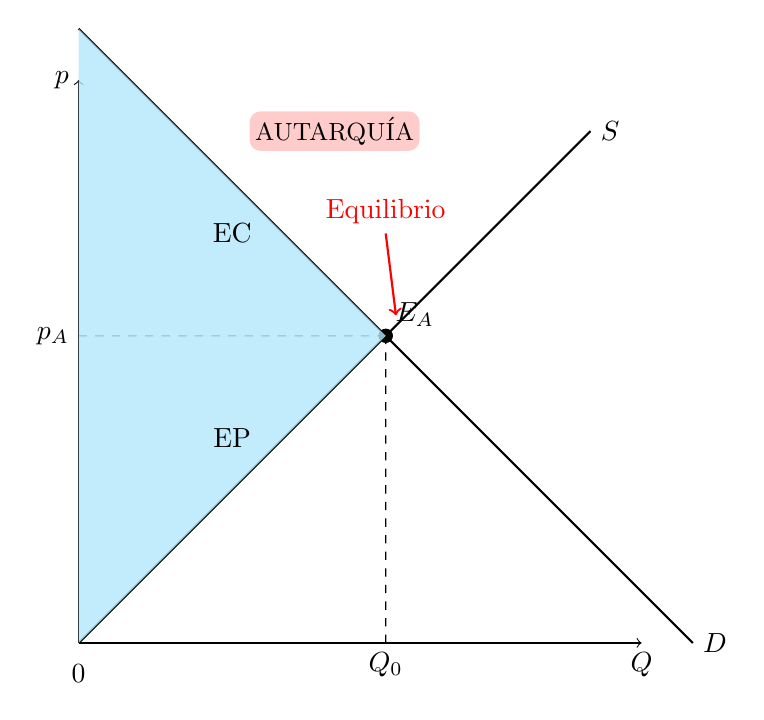
\begin{tikzpicture}[scale=1.3]
    % Titulo
    \node[fill=red!20, text=black, rounded corners, inner sep=2pt, font=\small] at (2.5, 5) {AUTARQUÍA};

    % Ejes
    \draw[->] (0,0) -- (5.5,0) node[below] {$Q$};
    \draw[->] (0,0) -- (0,5.5) node[left] {$p$};
    \node at (0, -0.3) {0};

    % Curvas de Oferta y Demanda (S=P, D=6-P)
    \draw[thick] (0, 0) -- (5, 5) node[right] {$S$}; % Oferta 
    \draw[thick] (0, 6) -- (6, 0) node[right] {$D$}; % Demanda
    
    % Punto de equilibrio en Autarquía (E_A)
    \def\pa{3} 
    \def\qa{3} 
    
    \coordinate (EA) at (\qa, \pa); % Punto de Autarquía
    \draw[dashed] (0, \pa) node[left] {$p_A$} -- (EA);
    \draw[dashed] (EA) -- (\qa, 0) node[below] {$Q_0$};
    \fill (EA) circle (2pt);
    \node[above right] at (EA) {$E_A$};
    
    % Flecha de Equilibrio
    \draw[->, thick, red] (3, 4) -- (3.1, 3.2);
    \node[above, red] at (3, 4) {Equilibrio};

    % Áreas de Excedente
    \coordinate (yInterceptD) at (0, 6);
    \coordinate (origin) at (0, 0);
    
    % Excedente del Consumidor (EC)
    \fill[cyan!30, opacity=0.8] (yInterceptD) -- (EA) -- (0, \pa) -- cycle;
    \node at (1.5, 4) {EC};
    
    % Excedente del Productor (EP)
    \fill[cyan!30, opacity=0.8] (origin) -- (EA) -- (0, \pa) -- cycle;
    \node at (1.5, 2) {EP};

\end{tikzpicture}
\hspace{1cm} % Espacio entre los dos gráficos
% Gráfico de la Derecha: LIBRE COMERCIO
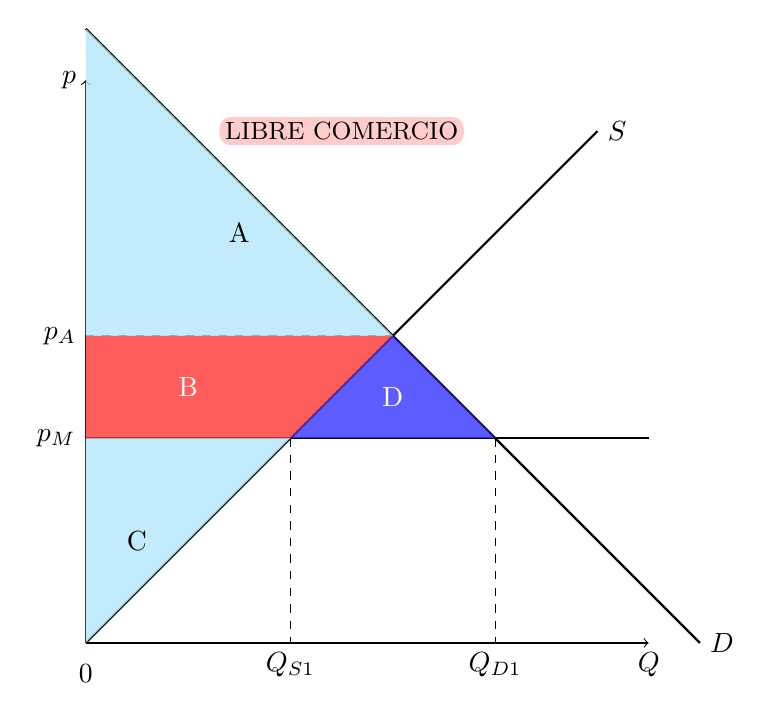
\begin{tikzpicture}[scale=1.3]
    % Titulo
    \node[fill=red!20, text=black, rounded corners, inner sep=2pt, font=\small] at (2.5, 5) {LIBRE COMERCIO};

    % Ejes
    \draw[->] (0,0) -- (5.5,0) node[below] {$Q$};
    \draw[->] (0,0) -- (0,5.5) node[left] {$p$};
    \node at (0, -0.3) {0};

    % Curvas de Oferta y Demanda
    \draw[thick] (0, 0) -- (5, 5) node[right] {$S$}; % Oferta 
    \draw[thick] (0, 6) -- (6, 0) node[right] {$D$}; % Demanda
    
    % Precios de Autarquía y Mundial
    \def\pa{3}
    \def\pm{2} % Precio Mundial (P_M)
    
    \draw[dashed] (0, \pa) node[left] {$p_A$} -- (3, \pa);
    \draw[thick] (0, \pm) node[left] {$p_M$} -- (5.5, \pm);
    
    % Cantidades
    \def\qs{2} % Q_S1 (Producción doméstica)
    \def\qd{4} % Q_D1 (Consumo doméstico)
    
    \draw[dashed] (\qs, \pm) -- (\qs, 0) node[below] {$Q_{S1}$};
    \draw[dashed] (\qd, \pm) -- (\qd, 0) node[below] {$Q_{D1}$};
    
    % Coordenadas para las áreas
    \coordinate (EA) at (3, \pa);
    \coordinate (yInterceptD) at (0, 6);
    \coordinate (origin) at (0, 0);
    \coordinate (Qs_pm) at (\qs, \pm);
    \coordinate (Qd_pm) at (\qd, \pm);
    
    % Área A (Excedente Consumidor remanente)
    \fill[cyan!30, opacity=0.8] (yInterceptD) -- (EA) -- (0, \pa) -- cycle;
    \node[text=black] at (1.5, 4) {A};

    % Área B (Transferencia de EP a EC)
    \fill[red!80, opacity=0.8] (0, \pa) -- (EA) -- (Qs_pm) -- (0, \pm) -- cycle;
    \node[text=white] at (1, 2.5) {B};
    
    % Área C (Excedente Productor remanente)
    \fill[cyan!30, opacity=0.8] (origin) -- (Qs_pm) -- (0, \pm) -- cycle;
    \node[text=black] at (0.5, 1) {C};
    
    % Área D (Ganancia neta de bienestar)
    \fill[blue!80, opacity=0.8] (EA) -- (Qd_pm) -- (Qs_pm) -- cycle;
    \node[text=white] at (3, 2.4) {D};
    
\end{tikzpicture}
\caption{Comparación del bienestar en autarquía y libre comercio para un país importador.}
\end{figure}

\subsection{La Demanda de Importaciones }

La \textbf{curva de demanda de importaciones} ($M$) es una herramienta conceptual clave que se deriva de las curvas de oferta ($S$) y demanda ($D$) domésticas de un país . La demanda de importaciones se define como el \textbf{exceso} de lo que los consumidores nacionales demandan sobre lo que los productores nacionales ofrecen, dado un precio internacional .

$$M = D - S \quad \text{(a un precio dado)}$$

La curva de demanda de importaciones es \textbf{decreciente} respecto al precio. En el punto de autarquía ($p_A$), la demanda de importaciones es cero ($D=S$) . A medida que el precio internacional desciende por debajo de $p_A$, la demanda doméstica de importaciones se vuelve positiva y aumenta, ya que el consumo aumenta y la producción nacional disminuye .

\subsubsection{Deducción Gráfica de la Demanda de Importaciones}

El gráfico mediante \texttt{TikZ} ilustra cómo la diferencia entre la demanda interna y la oferta interna a distintos precios (Panel (a)) define la curva de demanda de importaciones (Panel (b)) .

\begin{figure}[h]
\centering
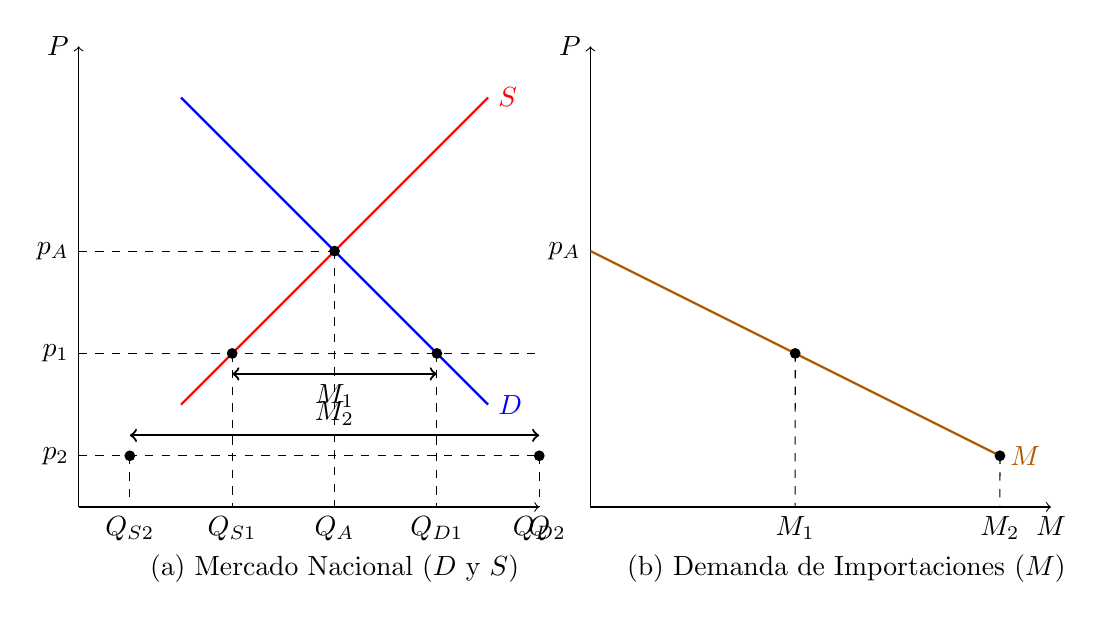
\begin{tikzpicture}[scale=1.3]

    % Panel A: Mercado Nacional (Oferta y Demanda)
    \begin{scope}[shift={(0,0)}]
        \draw[->] (0,0) -- (4.5,0) node[below] {$Q$};
        \draw[->] (0,0) -- (0,4.5) node[left] {$P$};

        % Curvas de Oferta y Demanda 
        \draw[blue, thick] (1, 4) -- (4, 1) node[right] {$D$}; % Demanda
        \draw[red, thick] (1, 1) -- (4, 4) node[right] {$S$}; % Oferta

        % Precio de Autarquía (P_A = 2.5, Q_A = 2.5)
        \def\pa{2.5}
        \draw[dashed] (0, \pa) node[left] {$p_A$} -- (2.5, \pa);
        \draw[dashed] (2.5, \pa) -- (2.5, 0) node[below] {$Q_A$};
        \fill (2.5, \pa) circle (1.5pt);

        % Precio 1 (p_1 < p_A)
        \def\pUno{1.5}
        \draw[dashed] (0, \pUno) node[left] {$p_1$} -- (4.5, \pUno);
        % En P1, Qs < Q_A < Qd
        \def\qsUno{1.5} \def\qdUno{3.5}
        \draw[dashed] (\qsUno, 0) node[below] {$Q_{S1}$};
        \draw[dashed] (\qdUno, 0) node[below] {$Q_{D1}$};
        \draw[dashed] (\qsUno, \pUno) -- (\qsUno, 0);
        \draw[dashed] (\qdUno, \pUno) -- (\qdUno, 0);
        \draw[<->, thick] (\qsUno, \pUno - 0.2) -- (\qdUno, \pUno - 0.2) node[midway, below] {$M_1$};
        \fill (\qsUno, \pUno) circle (1.5pt); \fill (\qdUno, \pUno) circle (1.5pt);

        % Precio 2 (p_2 < p_1)
        \def\pDos{0.5}
        \draw[dashed] (0, \pDos) node[left] {$p_2$} -- (4.5, \pDos);
        % En P2, Qs < Qs1 < Qd1 < Qd
        \def\qsDos{0.5} \def\qdDos{4.5}
        \draw[dashed] (\qsDos, 0) node[below] {$Q_{S2}$};
        \draw[dashed] (\qdDos, 0) node[below] {$Q_{D2}$};
        \draw[dashed] (\qsDos, \pDos) -- (\qsDos, 0);
        \draw[dashed] (\qdDos, \pDos) -- (\qdDos, 0);
        \draw[<->, thick] (\qsDos, \pDos + 0.2) -- (\qdDos, \pDos + 0.2) node[midway, above] {$M_2$};
        \fill (\qsDos, \pDos) circle (1.5pt); \fill (\qdDos, \pDos) circle (1.5pt);

        \node at (2.5, -0.6) {(a) Mercado Nacional ($D$ y $S$)};
    \end{scope}

    % Panel B: Curva de Demanda de Importaciones (M)
    \begin{scope}[shift={(5,0)}]
        \draw[->] (0,0) -- (4.5,0) node[below] {$M$};
        \draw[->] (0,0) -- (0,4.5) node[left] {$P$};
        
        % Punto de intersección M=0 (P_A)
        \draw[dashed] (0, \pa) node[left] {$p_A$};
        
        % Curva de Demanda de Importaciones (M)
        % M es una función decreciente. M1=QD1-QS1=2. M2=QD2-QS2=4.
        \coordinate (M_pA) at (0, \pa);
        \coordinate (M_p1) at (2, \pUno); 
        \coordinate (M_p2) at (4, \pDos); 

        % Dibujar M (aproximando curva a los puntos)
        \draw[orange!70!black, thick] (M_pA) -- (M_p1) -- (M_p2) node[right] {$M$};
        
        % Trazado de puntos M1 y M2
        \draw[dashed] (M_p1) -- (2, 0) node[below] {$M_1$};
        \draw[dashed] (M_p2) -- (4, 0) node[below] {$M_2$};
        \fill (M_p1) circle (1.5pt);
        \fill (M_p2) circle (1.5pt);

        \node at (2.5, -0.6) {(b) Demanda de Importaciones ($M$)};
    \end{scope}

\end{tikzpicture}
\caption{Deducción de la Curva de Demanda de Importaciones}
\end{figure}

\paragraph{Explicación del gráfico:}
\begin{enumerate}
    \item \textbf{Panel (a)}: Muestra la oferta ($S$) y la demanda ($D$) doméstica. En el precio de autarquía ($p_A$), la demanda de importaciones ($M$) es cero. Cuando el precio cae a $p_1$ y luego a $p_2$, la demanda doméstica excede a la oferta doméstica, creando un exceso de demanda (Importaciones, $M$) que aumenta de $M_1$ a $M_2$ .
    \item \textbf{Panel (b)}: La curva de demanda de importaciones ($M$) refleja la relación inversa entre el precio y la cantidad de importaciones deseadas, derivada directamente de los excesos de demanda observados en el mercado nacional. Esta curva comienza en $p_A$ (donde $M=0$) y se extiende hacia la derecha a medida que el precio disminuye .
\end{enumerate}

\subsection{Ganancias Adicionales del Libre Comercio}
Más allá de las ganancias estáticas derivadas de la reasignación eficiente de los recursos según la ventaja comparativa , el libre comercio ofrece \textbf{beneficios adicionales} (o dinámicos) que enriquecen el bienestar nacional y que son difíciles de cuantificar en un análisis coste-beneficio convencional .

Entre estos beneficios adicionales se encuentran:
\begin{enumerate}
    \item \textbf{Economías de Escala y Eficiencia}: El libre comercio incrementa el tamaño del mercado para las empresas nacionales, lo que les permite \textbf{explotar economías de escala} y alcanzar niveles de producción más eficientes, reduciendo los costes unitarios . Esto es crucial para países pequeños o medianos .
    \item \textbf{Aumento de la Competencia y la Innovación}: El libre comercio intensifica la competencia a nivel nacional, lo que incentiva a las empresas a \textbf{buscar nuevas vías para exportar e innovar} . Esto fomenta un aumento de la productividad y una mayor diversidad de productos para los consumidores . La exposición a la competencia global obliga a las industrias a mejorar su eficiencia y a reasignar recursos de usos de baja productividad a usos de alta productividad .
    \item \textbf{Mejora de la Relación de Intercambio (desde la perspectiva dinámica)}: El comercio promueve el crecimiento económico a largo plazo, lo que genera \textbf{ganancias dinámicas} que se suman a las ganancias estáticas por la reasignación de recursos existentes .
\end{enumerate}

Estos argumentos, junto con la \textbf{perspectiva de la economía política} (que ve el libre comercio como una herramienta para contrarrestar la presión de grupos de interés en favor del proteccionismo) , refuerzan la posición de que el libre comercio es el ideal por el cual la política comercial debe luchar .





%===========================================
%===========================================

% APUNTES CLASE

%===========================================
%===========================================

\section{Las cuotas de la importación en un país pequeño}


¿Cuál es el efecto de la cuota a la importación sobre el bienestar de nación?

El efecto de una cuota a la importación sobre el bienestar nacional en un país pequeño es, en términos generales, negativo. Al limitar la cantidad de bienes que pueden importarse, la cuota eleva el precio interno del bien protegido, lo que reduce el excedente del consumidor y genera una transferencia de ingresos hacia los productores nacionales y los titulares de licencias de importación. Sin embargo, la suma de las pérdidas de eficiencia (por reducción del consumo y producción ineficiente) supera las ganancias de los beneficiarios directos, resultando en una pérdida neta de bienestar nacional equivalente a las áreas de pérdida de eficiencia (\(B + D\)) en el análisis gráfico estándar. Además, si las licencias de importación se asignan mediante mecanismos no competitivos (por ejemplo, favoritismo o corrupción), pueden surgir costes adicionales asociados a la búsqueda de rentas, incrementando aún más la pérdida de bienestar.

% Mecanismo de licencias a la importación:

% Búsqueda de rentas: es el soborno o la creación de grupos de presión que aspiran a la obtenicón de licencias a la importación ello le permitirña obtener la renta de cuota de importación.

% Efecto de rentas de la cuota -> 0: pues quienes poseen licencia importación estarían dispuestos a pagar máximo.

\subsection{Efectos de una cuota de importación en un país pequeño}

Los efectos de una cuota de importación sobre el bienestar nacional pueden desglosarse en los siguientes componentes:

\begin{itemize}
    \item \textbf{Efecto sobre el consumo}: Reducción del bienestar de los consumidores debido al aumento del precio interno y la disminución de la cantidad consumida. -(A+B+C+D)
    \item \textbf{Efecto sobre la producción}: Beneficio para los productores nacionales, que pueden vender a un precio más alto y aumentar su producción. +A
    \item \textbf{Efecto de renta de la cuota}: Las rentas generadas por la cuota son percibidas por quienes obtienen las licencias de importación, ya que pueden importar y vender la cantidad permitida a un precio superior al precio mundial. 0
    \item \textbf{Efecto neto sobre el bienestar nacional}: La suma de los efectos anteriores se traduce en una pérdida de bienestar equivalente a las áreas de pérdida de eficiencia (\(B + D\)), donde \(B\) representa la pérdida por consumo y \(D\) la pérdida por producción. E.consumo + E.producción + E.rentaCuota.
\end{itemize}


\section{Necanismo de asignacion de las cuotas de importación}


% SUbasta de cuotas: los gobiernos pueden sbastar las licencias de cuota a la importación

% ¿Cuál es el efecto en el bienestar de las cuotas de importación?


% Restricciones voluntarias de la exportación o cuotas: el gobierno de un paós limira las unidades exportadas a inciiativa propiaa asignando a las empresas exportadoras una cuota de exportación

% Efecto cuota -> 0: ya que las rentas si las hay , las perciben las emppresas del país que exporta.


\subsection{Subasta de cuotas}

Los gobiernos pueden asignar las licencias de cuota de importación mediante subasta. En este mecanismo, las empresas interesadas pujan por el derecho a importar bajo la cuota, y las licencias se otorgan a quienes ofrecen el mayor precio. Este procedimiento permite que el Estado capture las rentas generadas por la cuota, en lugar de que sean apropiadas por los titulares privados de las licencias.

\textbf{Efecto sobre el bienestar:} La subasta de cuotas elimina la renta privada asociada a la cuota, transfiriéndola al gobierno. Sin embargo, la pérdida de eficiencia (\(B + D\)) persiste, por lo que el efecto neto sobre el bienestar nacional sigue siendo negativo.

\subsection{Restricciones Voluntarias a la Exportación (RVE)}

Las restricciones voluntarias a la exportación son acuerdos mediante los cuales el gobierno de un país exportador limita, por iniciativa propia, la cantidad de bienes exportados, asignando cuotas de exportación a sus empresas.

\textbf{Efecto sobre el bienestar:} En este caso, las rentas generadas por la restricción son capturadas por las empresas exportadoras del país extranjero, no por el país importador. Por tanto, el efecto de renta para el país importador es nulo, y la pérdida de eficiencia (\(B + D\)) permanece.


% Restricciones voluntarias de la exportación o cuotas 
% En este caso el efecto neto dsobre el nienestar nacñin seria -(B+C+D)


\subsection{Efecto de las Restricciones Voluntarias a la Exportación (RVE) sobre el Bienestar Nacional}

Cuando se implementan restricciones voluntarias a la exportación (RVE), el efecto neto sobre el bienestar nacional del país importador es negativo. Específicamente, la pérdida de bienestar equivale a las áreas \(B + C + D\) en el análisis gráfico estándar, donde:

\begin{itemize}
    \item \(B\): Pérdida por consumo debido al aumento de precios y reducción de la cantidad consumida.
    \item \(C\): Transferencia de renta a las empresas exportadoras extranjeras, ya que son ellas quienes capturan las rentas generadas por la restricción.
    \item \(D\): Pérdida por producción ineficiente, al incentivar la producción nacional a un coste mayor que el internacional.
\end{itemize}

Por tanto, bajo una RVE, el país importador no recibe las rentas de la cuota, y la suma de las pérdidas de eficiencia y la transferencia de renta resulta en una disminución del bienestar nacional igual a \(- (B + C + D)\).

\subsection{Subsidio a la Exportación}

Un \textbf{subsidio a la exportación} es un pago realizado por el gobierno a las empresas que exportan bienes, con el objetivo de fomentar las ventas internacionales. Existen principalmente dos tipos de subsidios a la exportación:

\begin{itemize}
    \item \textbf{Subsidio ad valorem}: Se expresa como un porcentaje fijo del valor exportado.
    \item \textbf{Subsidio específico}: Se otorga como una cantidad fija por unidad exportada.
\end{itemize}

El efecto de un subsidio a la exportación sobre el precio puede representarse como:

\[
p_m + s = \text{precio mundial}
\]

donde \(p_m\) es el precio interno antes del subsidio y \(s\) es el monto del subsidio otorgado por unidad exportada.



